% !TEX program = xelatex
\documentclass[12pt,a4paper]{ctexart}

\usepackage[margin=2.3cm]{geometry}
\usepackage{amsmath,amssymb}
\usepackage{graphicx}
\usepackage{booktabs}
\usepackage{longtable}
\usepackage{array}
\usepackage{caption}
\usepackage{enumitem}
\usepackage{pifont}
\usepackage[colorlinks=true,linkcolor=blue!60!black,urlcolor=blue!60!black]{hyperref}
\usepackage{titlesec}
\usepackage{fancyvrb}

\captionsetup{font=small,labelfont=bf}
\titleformat{\section}{\large\bfseries}{\thesection}{0.6em}{}
\titleformat{\subsection}{\normalsize\bfseries}{\thesubsection}{0.6em}{}
\setlist{nosep,leftmargin=1.8em}
\renewcommand{\arraystretch}{1.15}
\graphicspath{{figures/}{../figures/}}
\setlength{\emergencystretch}{1.2em}

\title{\bfseries 2026 年高教社杯全国大学生数学建模竞赛 C 题\\[4pt]
问题 1 —— 两方案（DeepSeek 版 / GLM-5.3 版）对比与改进报告\\[6pt]
\large 微网与外部电网电力调控策略 —— 单日计划购电策略的优化模型}
\author{}
\date{}

\begin{document}
\maketitle
\vspace{-2.2cm}

\begin{center}
\begin{minipage}{0.93\textwidth}
\small
\textbf{本报告做的事：} 把两份外部解答（DeepSeek 版、GLM-5.3 版）的代码\textbf{逐字复现并实跑}，
逐项对比其建模、求解、输出与缺陷，给出经独立实现验证的统一结论，并说明本成果包对两份方案
分别做了哪些修正。
\end{minipage}
\end{center}

\section*{0\quad 结论速览}
\addcontentsline{toc}{section}{0\quad 结论速览}

\begin{center}
\begin{tabular}{@{}p{5.0cm} p{10.2cm}@{}}
\toprule
结论 & 内容 \\
\midrule
两份方案的模型是否都正确 & \textbf{都是}（数学上等价，最优值一致到 $10^{-6}$ 元）\\
两份方案的代码能否直接跑通 & \textbf{都能}（DeepSeek 版 HiGHS 秒级；GLM 版 PuLP+CBC 0.91 秒）\\
导出 result1.xlsx 是否合规 & \textbf{都不合规}（表头、时间列、充放电量表结构均不符附件 5 模板）\\
最终最优解（四方一致） & \textbf{全天购电量 59\,482.6990 kWh，全天购电费 35\,126.9486 元}\\
与无储能方案相比 & 节约 \textbf{12\,925.0980 元（26.90\%）}，弃光 6\,247.9630 $\to$ \textbf{0} kWh，
                     消纳率 88.7\% $\to$ \textbf{100\%}\\
\bottomrule
\end{tabular}
\end{center}

\textbf{两方案一句话评价：}
\begin{itemize}
  \item \textbf{DeepSeek 版}：模型框架正确但\textbf{论证最薄弱} —— 缺弃光变量、时标与表 1 索引自相矛盾、无任何数值结果与校验。
  \item \textbf{GLM-5.3 版}：方法论\textbf{明显更成熟} —— 明确提出"时段末端"约定、主动引入弃电变量、主动建议效率口径敏感性；但\textbf{弃电变量缺上界}，且导出的结果文件不合模板。
\end{itemize}

\section{两方案来源与复现验证}

两份方案都是针对同一微网经济调度问题\cite{lasseter,katiraei,wang}给出的单日优化解答，
本节先把它们的代码逐字复现并实跑。

\subsection{来源与复现方式}

\begin{center}
\small
\begin{tabular}{@{}p{2.4cm} p{6.4cm} p{6.4cm}@{}}
\toprule
项目 & 方案 A（DeepSeek 版） & 方案 B（GLM-5.3 版） \\
\midrule
原始材料 & \texttt{2026高教社杯 C题第一问解答.pdf}（8 页） & \texttt{新建 文本文档.txt}（GLM-5.3，8 节）\\
复现脚本 & \texttt{04\_原始方案与复现证据/DeepSeek\_方案代码复现.py} & \texttt{03\_方案B.../02\_代码/glm\_q1\_original.py}\\
复现改动 & 仅把附件路径改为绝对路径、输出目录改到 \texttt{results/} & 同 \\
指定求解器 & \texttt{scipy.optimize.linprog}（原文未指明，实为 HiGHS） & \texttt{PuLP} $+$ \texttt{PULP\_CBC\_CMD}\\
\bottomrule
\end{tabular}
\end{center}

\subsection{复现结果}

\textbf{方案 A（DeepSeek 版）实跑输出：}

\begin{quote}\ttfamily\small
全天购电量: 59482.6990 kWh\\
全天购电费: 35126.9486 元\\
{[}审计{]} 功率平衡 max|residual| = 1.819e-12 kW\\
{[}审计{]} 储能动态 max|residual| = 4.547e-13 kWh\\
{[}审计{]} 储电量范围 [1200.0000, 10800.0000]，E\_T = 6000.0000\\
{[}审计{]} 购电为负的时段数 = 0\\
{[}审计{]} 同时充放时段数 = 0\\
{[}审计{]} $\Sigma$max(0,-net)*dt = 6247.9630 kWh（中午富余总量，被迫由储能全额消纳）
\end{quote}

\textbf{方案 B（GLM-5.3 版）实跑输出：}

\begin{quote}\ttfamily\small
状态: Optimal\\
全天购电量=59,482.6990 kWh\quad 全天购电费=35,126.9486 元\\
弃电总量=0.0000 kWh；同时充放max(c·f)=0.00e+00\\
SOC范围[1200.00,10800.00]，E24=6000.00
\end{quote}

\textbf{两份方案的代码都无需修改即可跑通，且最优值与独立实现完全一致。}

\subsection{四方交叉验证}

\begin{center}
\footnotesize
\begin{tabular}{@{}p{3.5cm} p{3.2cm} r r r@{}}
\toprule
实现 & 求解器 & 全天购电量 (kWh) & 全天购电费 (元) & 平衡残差 (kW) \\
\midrule
方案 A 原始代码 & scipy / HiGHS & 59\,482.6990 & 35\,126.948589 & $1.82\times10^{-12}$\\
方案 B 原始代码 & PuLP / CBC & 59\,482.6990 & 35\,126.948591 & $4.00\times10^{-5}$\\
本包·方案 A 改进版 & scipy / HiGHS & 59\,482.6990 & 35\,126.948589 & $1.8\times10^{-12}$\\
本包·方案 B 改进版 & PuLP / CBC $+$ HiGHS & 59\,482.6990 & 35\,126.948591 & $1.8\times10^{-12}$\\
\bottomrule
\end{tabular}
\end{center}

\noindent\footnotesize 注：残差列取各实现原生求解器的结果；「本包·方案 B 改进版」同时提供
PuLP/CBC 与 scipy/HiGHS 两条路线，此处列 HiGHS 结果（CBC 为 $4.0\times10^{-5}$ kW）。

\textbf{四套独立实现、两类求解器，得到同一个最优值} —— 这是对模型与结果最有力的交叉验证。

\section{建模方案逐项对比}

\subsection{对比总表}

\begin{longtable}{@{}p{2.5cm} p{4.2cm} p{4.3cm} p{4.2cm}@{}}
\toprule
维度 & 方案 A（DeepSeek） & 方案 B（GLM-5.3） & 本包处理 \\
\midrule
\endhead
问题识别 & 单日确定性 LP \ding{51} & 单日确定性 LP \ding{51} & 一致\\
决策变量 & $P^{buy},P^{ch},P^{dis},E$（$4\times144=576$） & $p,c,f,d,E$（$5\times144=720$） & 采用 $5\times144$\\
目标函数 & $\min\sum c_tP_t^{buy}\Delta t$ \ding{51} & $\min\sum\pi_tp_t\Delta t$ \ding{51} & 一致\\
弃光/弃电变量 & \textbf{无} \ding{55} & 有 $d_t\ge0$（\textbf{缺上界}）\ding{56} & 有 $0\le d_t\le v_t$ \ding{51}\\
时标语义 & 表述含糊、\textbf{索引自相矛盾} \ding{55} & \textbf{"时段末端"（正确）} \ding{51} & 同 B \ding{51}\\
表 1 索引 & 取 $t=60$ $\to$ 实际是 9:50--10:00 \ding{55} & idx=[60,72,…]（0-based）\ding{51} & 同 B \ding{51}\\
充放电效率 & 双侧 0.9/0.9 & 双侧 0.9/0.9 \textbf{$+$ 建议单侧口径敏感性} \ding{51} & 参数化，支持 3 种口径 \ding{51}\\
首尾储电量 & $E_0=E_{144}=6000$ \ding{51} & 同 \ding{51} & 同 \ding{51}\\
充放电互斥 & 断言"LP 不需要"，\textbf{未论证} & 断言"互补松弛"，\textbf{用词不准} & 给出严格证明 \ding{51}\\
储能净损耗机理 & 未讨论 \ding{55} & 未讨论 \ding{55} & 给出严格论证 \ding{51}\\
约束冗余 & \texttt{A\_ub} 与 \texttt{bounds} 重复 576 行 \ding{55} & 无 \ding{51} & 无 \ding{51}\\
模型规模描述 & 未给出 & "约 440 条"（\textbf{不准}）\ding{56} & 准确：289 等式 $+$ 720 界 \ding{51}\\
\bottomrule
\end{longtable}

\subsection{弃光/弃电变量（核心差异之一）}

\begin{itemize}
  \item \textbf{方案 A 完全没有}：功率平衡写作 $b_t+PV_t+d_t=L_t+g_t$，即\textbf{强制光伏全额消纳}，
        同时要求 $b_t\ge0$。当富余光伏超过储能吸收能力时模型\textbf{无可行解}。
        本题恰好可行：中午富余总量 6\,247.9630 kWh，储能单日可吸收
        $\eta_c(E_{\max}-E_{\min})=0.9\times9\,600=8\,640$ kWh $>$ 6\,247.9630 kWh。
        属于"侥幸可行"，原文对此毫无讨论。
  \item \textbf{方案 B 引入 $d_t$ 但缺上界}：只写 $d_t\ge0$。物理上弃电量不可能超过当时可用的
        光伏功率，缺上界意味着 $v_t=0$ 的时段也可能出现"弃电"，对任意输入不稳健。
        实测：本题最优解 $d^*\equiv0$，故\textbf{不影响数值结果}。
  \item \textbf{本包}：补 $0\le d_t\le v_t$，既保留可行性保障又保证物理严谨。
\end{itemize}

光伏富余的本地消纳是微网经济性的核心问题\cite{luthander}，而储能容量与功率配置直接决定光伏消纳能力\cite{storage}。

\subsection{时标语义与表 1 索引（核心差异之二）}

\textbf{附件 1 的采样时刻为 0:10, 0:20, \dots, 24:00。} 只有"采样时刻 $=$ 10 分钟区间的
\textbf{右端点}"这一解释，才能让 0:00 的储电量对应 $E_0$、24:00 的储电量对应 $E_{144}$，
与题目"0:00 与 24:00 储电量相同"自洽。若按左端点解释，全天覆盖区间将变成
$[0{:}10, 24{:}10)$，首尾各错位 10 分钟。

\begin{center}
\small
\begin{tabular}{@{}p{2.6cm} p{6.6cm} p{5.8cm}@{}}
\toprule
方案 & 表 1 取的行 & 与其自身时标表述是否一致 \\
\midrule
A（DeepSeek） & $t=60$（时刻 10:00）$\to$ \textbf{左端点口径} &
\textbf{不一致}：原文说"$t=1$ 对应 00:10"（右端点体系），却用 $t=60$ 表示 10:00--10:10 \\
B（GLM） & idx=[60,72,…]（0-based）$\to$ 1-based $t=61$（时刻 10:10）$\to$ \textbf{右端点口径} &
\textbf{一致} \ding{51} \\
\bottomrule
\end{tabular}
\end{center}

方案 B 在第八节还主动提示"若模板以 10:00 行起算，把 idx 改为 [59,71,…]，务必对照附件 5
模板确认"，但未给出最终判断；本包在 \S6 给出定论。

\subsection{效率口径}

两方案都采用\textbf{双侧 0.9}（往返 81\%），这一点一致且符合行业惯例。
\textbf{方案 B 额外提出应做"单侧 90\%"口径的敏感性分析} —— 这是方案 B 相对方案 A 的实质性
加分项，本包已落实（见 \S7.2）；分时电价机制是这类峰谷套利策略的制度基础\cite{price}，
效率口径对储能套利收益的影响可参考文献\cite{harsha}。

\subsection{"同时充放电"命题的论证}

两方案都断言 LP 最优解不含同时充放电，但都\textbf{没有给出正确论证}（方案 A 说"会因效率损失
增加成本"，方向对但未说清；方案 B 说"互补松弛"，用词错误 —— 这不是互补松弛，而是
\textbf{目标函数单调性}）。

\textbf{正确论证}（本包）：设某时段 $c_t>0$ 且 $f_t>0$，取 $\delta=\min(c_t,f_t/0.81)>0$，
令 $c_t'=c_t-\delta$、$f_t'=f_t-0.81\delta$，则储量动态不变，而由平衡式
\[
p_t'=L_t+c_t'-f_t'-v_t+d_t=p_t-0.19\,\delta<p_t,
\]
即购电量与费用同时下降，与最优性矛盾。\textbf{实测：两方案的解都满足"同时充放时段数 $=0$"。}

\section{求解器与数值精度对比}

两方案分别使用 scipy/HiGHS\cite{scipy,highs} 与 PuLP/CBC\cite{pulp,cbc} 两类求解器，
故有必要对比其数值精度。

\begin{center}
\begin{tabular}{@{}l l l@{}}
\toprule
项目 & 方案 A（scipy / HiGHS） & 方案 B（PuLP / CBC） \\
\midrule
求解时间 & 秒级 & 约 0.91 秒 \\
功率平衡残差 & $\mathbf{1.82\times10^{-12}}$ kW & $4.00\times10^{-5}$ kW \\
储能动态残差 & $\mathbf{4.55\times10^{-13}}$ kWh & $4.70\times10^{-4}$ kWh \\
收紧容差（$10^{-9}$）是否改善 & --- & \textbf{无改善} \\
目标值 & 35\,126.948589 元 & 35\,126.948591 元 \\
表 1 六值（6 位小数） & 一致 & 一致 \\
\bottomrule
\end{tabular}
\end{center}

\noindent\footnotesize 注：CBC 在默认容差与收紧到 $10^{-9}$ 时结果完全相同，说明 $10^{-5}$ 量级的残差并非容差参数所致。

\textbf{结论：} CBC 的解在数值上有 $10^{-5}$ 量级的约束残差，且与求解器容差参数无关；
但\textbf{表 1 的六个值在两种求解器下 6 位小数完全一致}，对四位小数的提交结果无影响。
若需更高数值保证（例如做对偶分析），建议用 HiGHS 或 GLPK。

\section{输出文件合规性对比}

题目明确要求"模板文件见附件 5"，两份方案都\textbf{未按模板填写}：

\begin{center}
\small
\begin{tabular}{@{}p{3.6cm} p{3.9cm} p{3.9cm} p{3.9cm}@{}}
\toprule
检查项 & 官方模板 & 方案 A 输出 & 方案 B 输出 \\
\midrule
工作表名 & \texttt{计划购电量}、\texttt{充放电量} & 同 \ding{51} & 同 \ding{51} \\
「计划购电量」表头 & \texttt{时间段}/\texttt{购电量} & \texttt{时间}/\texttt{购电量(kWh)} \ding{55} & \texttt{时间}/\texttt{购电量} \ding{55} \\
「计划购电量」A 列 & \texttt{0:10-0:20} … \texttt{0:00+1-0:10+1} & \texttt{00:10:00}、\texttt{23:50}、\texttt{0:00+1}（\textbf{类型混杂}）\ding{55} & 同 \ding{55} \\
「充放电量」表头 & \texttt{时间段}/\texttt{充电量}/\texttt{放电量}/\texttt{时刻}/\texttt{储电量}（5 列） & \texttt{时间段}/\texttt{充电量(kWh)}/\texttt{放电量(kWh)}（3 列）\ding{55} & 同 \ding{55} \\
「充放电量」行数 & 7 行 & 9 行 \ding{55} & 9 行 \ding{55} \\
0:00/24:00 储电量位置 & D/E 列 & A 列第 8/9 行 \ding{55} & 同 \ding{55} \\
\bottomrule
\end{tabular}
\end{center}

\textbf{两者导出的文件都无法直接提交。} 本包两个方案目录下的 \texttt{03\_结果/result1.xlsx}
均改为"拷贝附件 5 模板 $\to$ 只回填数值"的方式生成，并逐项校验（工作表名、表头、
A 列 144 个标签、维度、数值逐行）。

\section{缺陷清单对比}

\begin{center}
\begin{tabular}{@{}c p{6.2cm} p{6.2cm}@{}}
\toprule
编号 & 方案 A（DeepSeek） & 方案 B（GLM-5.3） \\
\midrule
D1 & 缺弃光/售电变量，可行性未论证 & \textbf{result1.xlsx 未套用附件 5 模板} \\
D2 & 时段编号与表 1 取值自相矛盾 & 弃电变量缺上界 $0\le d_t\le v_t$ \\
D3 & 界约束在 \texttt{bounds} 与 \texttt{A\_ub} 中重复（冗余 576 行） & CBC 解残差 $10^{-5}$ 量级（收紧容差无效）\\
D4 & 无任何数值结果与校验 & 约束规模"约 440 条"描述不准 \\
D5 & 无对照方案与经济性分析 & 只有"检验要点"清单，\textbf{未执行}校验/对照/图表 \\
D6 & 储能净损耗机理未讨论 & \texttt{tab1.loc[len(tab1)]} 健壮性差；"互补松弛"用词错误 \\
D7 & --- & 模板标签 10 分钟偏移只提示、未给结论 \\
\textbf{合计} & \textbf{6 项} & \textbf{7 项} \\
\bottomrule
\end{tabular}
\end{center}

两方案的缺陷\textbf{几乎不重叠}：方案 A 缺的是"模型严谨性与结果支撑"，方案 B 缺的是
"输出合规性与执行完备性"。

\section{关键分歧：时段口径（本包已定论）}

\subsection{分歧是什么}

附件 5 模板「计划购电量」工作表的 A 列首行标签是 \texttt{0:10-0:20}、末行是
\texttt{0:00+1-0:10+1}。而按 \S2.3 的"右端点"约定，第 $t$ 个时段覆盖 $(10(t-1),10t]$，
第一段应为 \texttt{0:00-0:10}。

\textbf{模板标签相对其实际覆盖区间整体晚了 10 分钟。} 证据：模板共 144 行数据，若首行真是
\texttt{0:10-0:20}，末尾将覆盖到次日 0:10，与题目"0:00 与 24:00 储电量相同"矛盾。

\subsection{两种取法给出的表 1 数值不同}

\begin{center}
\begin{tabular}{@{}l r r@{}}
\toprule
表 1 时间段 & 右端点口径 & 左端点口径 \\
 & （$t=61,73,85,97,109,121$） & （$t=60,72,84,96,108,120$） \\
\midrule
10:00-10:10 & 0.0000 & 0.0000 \\
12:00-12:10 & \textbf{480.4124} & \textbf{486.4029} \\
14:00-14:10 & 0.0000 & 0.0000 \\
16:00-16:10 & \textbf{445.4316} & \textbf{394.9315} \\
18:00-18:10 & \textbf{531.8940} & \textbf{636.9826} \\
20:00-20:10 & 0.0000 & 0.0000 \\
\midrule
全天购电量 & 59\,482.6990 kWh & 59\,482.6990 kWh \\
全天购电费 & 35\,126.9486 元 & 35\,126.9486 元 \\
\bottomrule
\end{tabular}
\end{center}

\noindent\small 全天总量与费用\textbf{不受影响}（两种口径只是"读同一份解的不同行"，解本身没变），
但表 1 的 6 个分时段数值差异最大达 \textbf{105 kWh}（18:00-18:10：531.89 vs 636.98）。

\begin{figure}[htbp]\centering
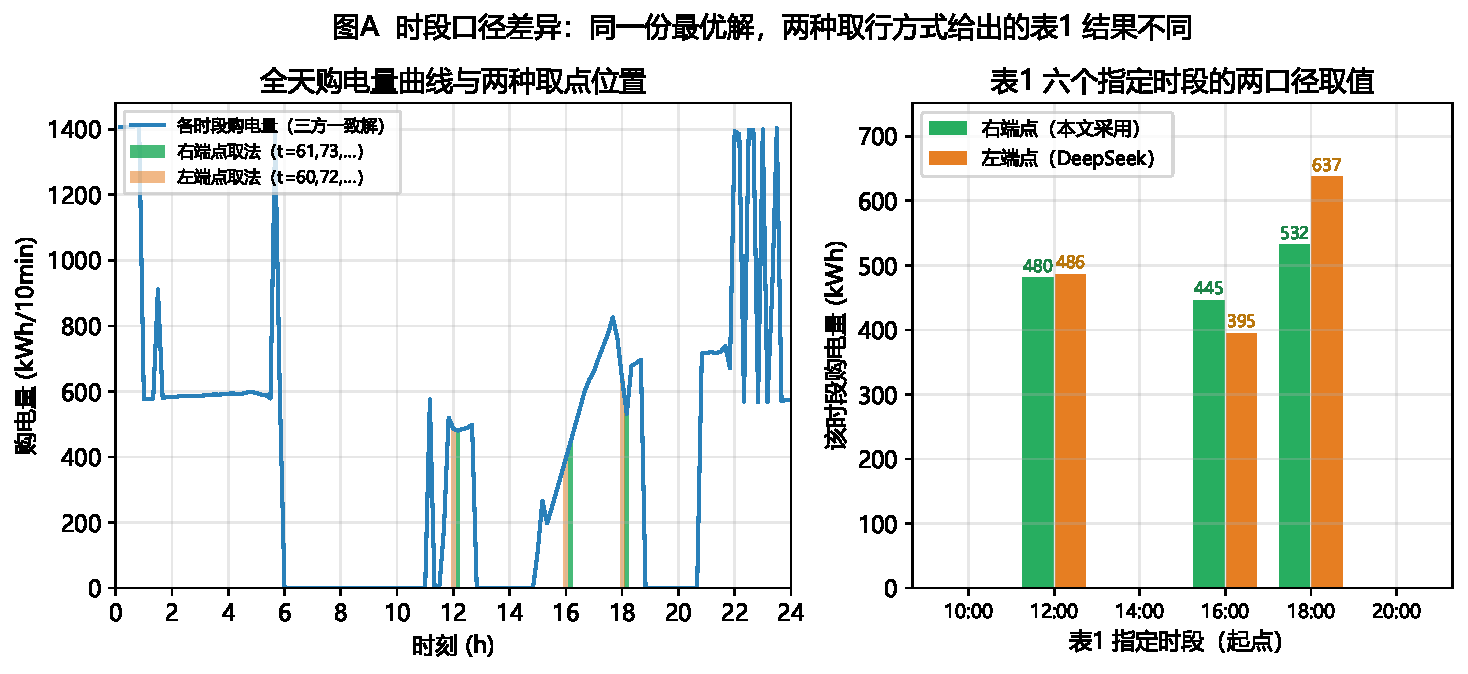
\includegraphics[width=0.95\textwidth]{figA_time_index.pdf}
\caption{时段口径差异：同一份最优解，两种取行方式给出的表 1 结果不同}
\end{figure}

\subsection{本包的处理}

\begin{enumerate}
  \item \textbf{论文表 1 采用右端点口径}（取 $t=61,73,85,97,109,121$）：这是唯一能让
        "0:00 储电量 $=E_0$、24:00 储电量 $=E_{144}$"与题目首尾约束自洽的约定，
        GLM 版也独立得出同一结论。
  \item \textbf{\texttt{result1.xlsx} 保持模板原标签不动，只回填 B 列数值}：第 $i$ 行的数值
        $=$ 第 $i$ 个时段的购电量，使数值序列与附件 1 行序严格一一对应，文件在形式上 100\%
        符合模板。
  \item \textbf{在报告中明示模板 A 列标签存在 10 分钟文本偏移}，使读者可以自行换算。
\end{enumerate}

\section{两方案共同缺失、由本包补齐的内容}

\subsection{独立校验}

对最优解执行 19 项校验并全部通过，其中与两方案缺陷直接对应的关键项：

\begin{center}
\begin{tabular}{@{}l p{9.6cm}@{}}
\toprule
校验 & 针对的缺陷 \\
\midrule
弃电界 $0\le d_t\le v_t$ & 方案 B 的 D2 \\
功率平衡 / 储能动态残差 & 两方案均未报告 \\
首尾储电量 $E_0=E_T=6000$ & 两方案均未数值验证 \\
充放电互斥（同时充放时段数 $=0$） & 两方案均只是断言 \\
result1.xlsx 模板合规性（5 项） & 两方案的 D1 \\
双求解器与跨实现交叉验证 & 两方案均未做 \\
\bottomrule
\end{tabular}
\end{center}

\subsection{效率口径敏感性（落实方案 B 的建议）}

\begin{center}
\begin{tabular}{@{}l c c r r@{}}
\toprule
口径 & $\eta_c/\eta_d$ & 往返效率 & 全天购电费 (元) & 相对主口径 \\
\midrule
\textbf{双侧 0.9/0.9（主口径）} & 0.9 / 0.9 & 81\% & \textbf{35\,126.95} & --- \\
单侧 0.9/1.0 & 0.9 / 1.0 & 90\% & 33\,416.53 & $-1\,710.42$（$-4.87\%$）\\
往返 90\% & 0.9487 / 0.9487 & 90\% & 33\,801.50 & $-1\,325.45$（$-3.77\%$）\\
\bottomrule
\end{tabular}
\end{center}

\textbf{值得注意：} 后两种口径的往返效率都是 90\%，购电费仍相差 385 元 —— 因为
\textbf{损耗发生在充电侧还是放电侧}会改变储能在高峰时段实际可释放的电量，进而改变最优调度。
因此\textbf{论文中必须明确 $\eta$ 的双侧口径}，并建议把单侧口径作为对照附表。

\subsection{无储能基准对照}

\begin{center}
\begin{tabular}{@{}l r r r r@{}}
\toprule
方案 & 全天购电量 (kWh) & 全天购电费 (元) & 弃光 (kWh) & 光伏消纳率 \\
\midrule
无储能 & 61\,789.9354 & 48\,052.0466 & 6\,247.9630 & 88.7\% \\
\textbf{有储能（最优）} & 59\,482.6990 & \textbf{35\,126.9486} & \textbf{0} & \textbf{100\%} \\
变化 & $-2\,307.2364$ & $\mathbf{-12\,925.0980\ (-26.90\%)}$ & $-6\,247.9630$ & $+11.3$ pp \\
\bottomrule
\end{tabular}
\end{center}

\subsection{储能配置敏感性}

\begin{minipage}[t]{0.49\textwidth}
\centering\footnotesize
\begin{tabular}{@{}r r r@{}}
\toprule
$P_{\max}$ (kW) & 购电费 (元) & 弃光 (kWh) \\
\midrule
0 & 48\,052.05 & 6\,247.96 \\
2\,500 & 36\,390.84 & 0 \\
\textbf{5\,000} & \textbf{35\,126.95} & \textbf{0} \\
7\,500 & 35\,027.13 & 0 \\
\bottomrule
\end{tabular}
\end{minipage}\hfill
\begin{minipage}[t]{0.49\textwidth}
\centering\footnotesize
\begin{tabular}{@{}r r r@{}}
\toprule
$E_{\max}$ (kWh) & 购电费 (元) & 弃光 (kWh) \\
\midrule
6\,000 & 40\,058.77 & 914.63 \\
8\,400 & 37\,165.01 & 0 \\
\textbf{10\,800} & \textbf{35\,126.95} & \textbf{0} \\
12\,000 & 34\,342.27 & 0 \\
\bottomrule
\end{tabular}
\end{minipage}

\vspace{0.8em}
\textbf{结论：} 功率 $\ge$2\,500 kW、容量 $\ge$7\,200 kWh 即可实现零弃光；费用随容量近似线性
下降，说明\textbf{容量（而非功率）是当前配置的主要瓶颈}（$E_{\max}$ 与 $E_{\min}$ 在最优解中
均被激活）。

\section{结论与使用建议}

\begin{enumerate}
  \item \textbf{两份方案的模型都是正确的}，且数学等价（方案 A 的强制全消纳在本题恰好等价于
        最优弃光为 0）。四套独立实现得到同一最优值 \textbf{35\,126.9486 元}，可以放心采用。
  \item \textbf{建议以方案 B（GLM-5.3）为基础}：它的时标语义、表 1 索引、弃电变量方向、
        效率口径意识都明显优于方案 A；再补上方案 B 缺失的 $0\le d_t\le v_t$、模板合规导出、
        校验与图表即可。
  \item \textbf{方案 A 有两点值得肯定}：约束"边界放在 \texttt{bounds}"的写法更简洁
        （虽然它在 \texttt{A\_ub} 里重复了）；以及它把常数项识别之外的模型结构写得较清楚。
  \item \textbf{必须注意}：两份方案\textbf{都没有给出任何数值校验}，也\textbf{都没有按附件 5
        模板导出结果文件}；本成果包已全部补齐。
  \item \textbf{时段口径是本问题最大的坑}：附件 5 模板 A 列标签相对实际区间晚 10 分钟。
        本包采用右端点口径（表 1 取第 61/73/85/97/109/121 行），并保持模板原标签、只回填数值
        —— 建议在论文中加一句脚注说明，避免评委误解。
\end{enumerate}

\begin{thebibliography}{99}
\small
\bibitem{problem} 全国大学生数学建模竞赛组委会. 2026 年高教社杯全国大学生数学建模竞赛 C 题：微网与外部电网电力调控策略[Z]. 2026.
\bibitem{format} 中国工业与应用数学学会. 全国大学生数学建模竞赛论文格式规范[Z]. 2026.
\bibitem{price} 国家发展和改革委员会. 关于进一步完善分时电价机制的通知（发改价格〔2021〕1093 号）[Z]. 2021-07-26.
\bibitem{storage} 国家发展和改革委员会, 国家能源局. 关于加快推动新型储能发展的指导意见（发改能源规〔2021〕1051 号）[Z]. 2021-07-15.
\bibitem{lasseter} Lasseter R H. MicroGrids[C]//IEEE Power Engineering Society Winter Meeting. New York: IEEE, 2002: 305-308.
\bibitem{katiraei} Katiraei F, Iravani R, Hatziargyriou N, et al. Microgrids management[J]. IEEE Power and Energy Magazine, 2008, 6(3): 54-65.
\bibitem{chen} Chen C, Duan S, Cai T, et al. Smart energy management system for optimal microgrid economic operation[J]. IET Renewable Power Generation, 2011, 5(3): 258-267.
\bibitem{harsha} Harsha P, Dahleh M. Optimal management and sizing of energy storage under dynamic pricing for the efficient integration of renewable energy[J]. IEEE Transactions on Power Systems, 2015, 30(3): 1164-1181.
\bibitem{luthander} Luthander R, Wid\'en J, Nilsson D, et al. Photovoltaic self-consumption in buildings: A review[J]. Applied Energy, 2015, 142: 80-94.
\bibitem{antonanzas} Antonanzas J, Osorio N, Escobar R, et al. Review of photovoltaic power forecasting[J]. Solar Energy, 2016, 136: 78-111.
\bibitem{wang} 王成山, 武震, 李鹏. 微电网关键技术研究[J]. 电工技术学报, 2014, 29(2): 1-12.
\bibitem{dantzig} Dantzig G B. Linear Programming and Extensions[M]. Princeton: Princeton University Press, 1963.
\bibitem{scipy} Virtanen P, Gommers R, Oliphant T E, et al. SciPy 1.0: fundamental algorithms for scientific computing in Python[J]. Nature Methods, 2020, 17(3): 261-272.
\bibitem{highs} Huangfu Q, Hall J A J. Parallelizing the dual revised simplex method[J]. Mathematical Programming Computation, 2018, 10(1): 119-142.
\bibitem{pulp} Mitchell S, O'Sullivan M, Dunning I. PuLP: A linear programming toolkit for Python[R]. Auckland: The University of Auckland, 2011.
\bibitem{cbc} Forrest J, Lougee-Heimer R. CBC user guide[C]//INFORMS Tutorials in Operations Research. 2005: 257-277.
\end{thebibliography}

\appendix
\section{本成果包结构}

\begin{quote}\ttfamily\small
00\_总览README.md\\
01\_两方案对比报告/ \quad $\leftarrow$ 本文档（$+$ PDF）\\
02\_方案A\_DeepSeek版\_审阅与改进/ \quad 01\_报告/ 02\_代码/ 03\_结果/ 04\_数据/\\
03\_方案B\_GLM5.3版\_审阅与改进/ \quad 00\_README.md 01\_报告/ 02\_代码/ 03\_结果/ 04\_数据/\\
04\_原始方案与复现证据/\\
\quad DeepSeek\_方案原文(文本提取).txt\\
\quad GLM5.3\_方案原文.txt\\
\quad DeepSeek\_方案代码复现.py \quad（逐字复现，仅改路径）\\
\quad DeepSeek\_原始输出\_result1.xlsx \quad（不合模板，对照用）\\
\quad GLM5.3\_原始输出\_result1.xlsx \quad（不合模板，对照用）\\
\quad 输出文件合规性审计.txt\\
\quad 两口径表1对照.json
\end{quote}

\subsection*{复现方式}
\begin{Verbatim}[fontsize=\small]
pip install numpy pandas scipy openpyxl matplotlib pulp

# 复现方案 A（DeepSeek）
python 04_原始方案与复现证据/DeepSeek_方案代码复现.py

# 复现方案 B（GLM-5.3）及其改进版
cd 03_方案B_GLM5.3版_审阅与改进/02_代码
python glm_q1_original.py    # 原始代码复现
python glm_solve.py          # 改进版求解 + 套模板导出
python glm_verify.py         # 19 项校验
python glm_sensitivity.py    # 19 组敏感性
python glm_figures.py        # 生成图表

# 方案 A 的改进版（独立实现）
cd ../../../02_方案A_DeepSeek版_审阅与改进/02_代码
python q1_solve.py && python q1_verify.py && python q1_sensitivity.py && python q1_figures.py
\end{Verbatim}

\end{document}
